\chapter{Micro}
\begin{figure}[!ht]
\begin{center}
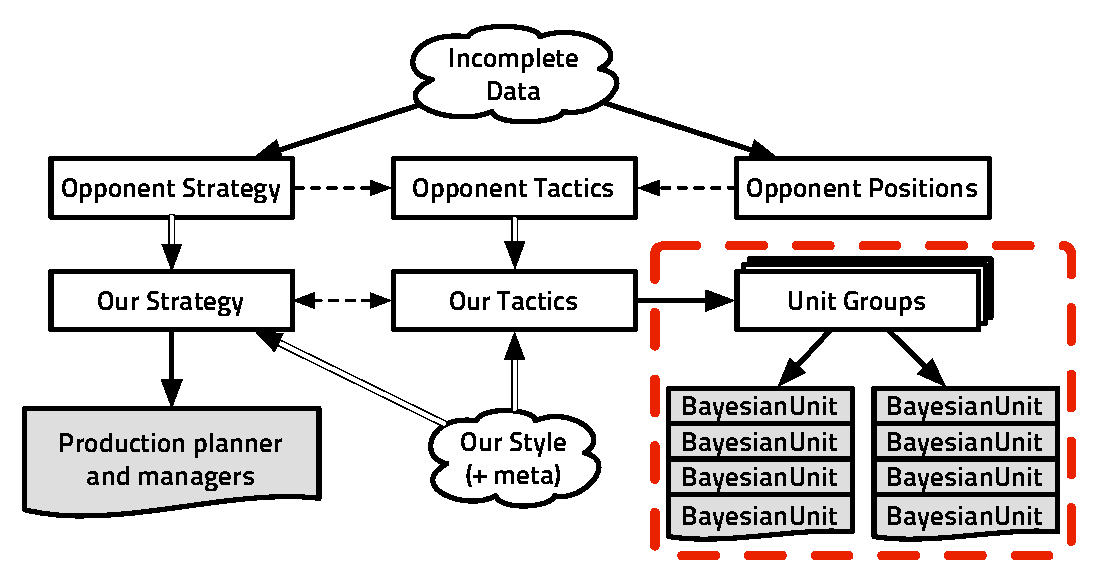
\includegraphics[width=13cm]{images/starcraft_bbq_concept_MICRO.pdf}
\end{center}
\label{fig:conceptMICRO}
\caption{Information-centric view of the architecture of the bot, the part concerning this chapter is in the dotted rectangle}
\end{figure}

\begin{itemize}
\item Problem: (optimal) control of units in a (real-continuous-time) huge actions space
\item Complexity: P-space
\item State of the art: de-centralized rules, \citep{Marthi05concurrenthierarchical}, \citep{WeberCIG10}
\item Our take: \citep{SYNNAEVE:Micro}
\item Results: more or less state of the art
\item Conclusion and perspectives: opens the game to parameters learning, RL and/or EA (Bayesian fusion FTW!)
\end{itemize}

